\documentclass[11pt, a4paper]{article}
\usepackage[utf8]{inputenc}
\usepackage[margin=1in]{geometry} %Sets proper 1-inch margins. 
\usepackage{amsmath} %Only load this if you are using math/equations.
\usepackage{graphicx} %Only need to call this if inserting images.
\usepackage{caption} %Only need to call this if inserting captions.
\usepackage{float} %Allows the use of the [H] specifier. 
\usepackage[colorlinks,citecolor=blue,linkcolor=blue,urlcolor=blue]{hyperref} %Allows for the embedding of urls. 
\usepackage{setspace}
\usepackage{blindtext}

\pagenumbering{arabic}

\usepackage{fancyhdr}

\pagestyle{fancy}
\fancyhf{}
\rhead{Jonah Edmundson \\ 2023}
\lhead{\thepage}

\newcommand{\comment}[1]{}

\usepackage{Sweave}
\begin{document}
\Sconcordance{concordance:regression.tex:regression.Rnw:%
1 22 1 1 0 20 1 1 12 1 8 4 1 1 5 3 0 1 1 41 0 1 3 1 4 3 0 1 10 1 0 1 2 %
2 1 1 11 1 1 1 5 14 0 1 2 4 1 1 4 2 2 3 0 1 1 8 0 1 2 6 1 1 5 1 1 1 5 3 %
0 1 1 40 0 1 3 1 5 3 0 1 10 1 0 1 2 2 1 1 11 1 1 1 6 14 0 1 2 4 1 1 4 1 %
2 9 1 1 5 1 3 1 1 1 5 3 0 1 1 13 0 1 5 2 0 1 11 1 0 1 2 9 1 1 6 1 4 49 %
0 1 2 1 1 1 5 3 0 1 11 1 0 1 2 7 1 1 8 25 0 1 3 2 0 1 10 1 0 1 2 6 1 1 %
6 15 0 1 2 1 1 1 10 1 4 3 0 1 10 1 0 1 2 7 1 1 4 11 0 1 2 1 1 1 4 3 0 1 %
11 1 0 1 2 7 1 1 4 3 0 1 1 12 0 1 2 1 4 3 0 1 10 1 0 1 2 10 1 1 3 3 0 1 %
10 4 0 1 2 18 1 1 5 38 0 1 3 1 5 3 0 1 10 1 0 1 2 2 1 1 5 14 0 1 2 6 1 %
1 6 1 4 49 0 1 2 1 1 1 5 3 0 1 11 1 0 1 2 7 1 1 8 25 0 1 3 2 0 1 10 1 0 %
1 2 4 1 1 5 14 0 1 2 1 1 1 10 1 4 3 0 1 10 1 0 1 2 7 1 1 3 11 0 1 2 1 1 %
1 4 3 0 1 11 1 0 1 2 7 1 1 3 3 0 1 1 12 0 1 2 1 4 3 0 1 10 1 0 1 2 10 1 %
1 3 3 0 1 10 4 0 1 2 18 1 1 3 1 2 7 1 1 3 1 2 9 1 1 3 1 2 10 1 1 30 3 0 %
1 1 6 0 1 1 14 0 1 1 2 0 1 1 6 0 1 1 14 0 1 10 1 0 1 2 11 1 1 2 3 0 1 %
15 1 0 1 2 11 1 1 7 3 0 1 2 4 0 1 3 1 0 1 2 12 1 1 14 7 0 1 1 14 0 1 3 %
1 0 1 2 9 1}


\begin{center}
\Large{\textsc{Regression Analysis}}
\par
\normalsize{\textsc{for}}
\par
\large{\textsc{Kelowna Weather-Crash Project}}
\end{center}


\vspace{0.917 pc} %Creates a paragraph line break. 

\tableofcontents



\pagebreak
\section{Predicting Number of Crashes}



\subsection{Simple Linear Regression}





\begin{Schunk}
\begin{Soutput}
Consistent Model Specification Test
Parametric null model: lm(formula = crashes ~ month + day + temp + relhum +
                          precip + wind.dir + wind.spd + visibility + pressure,
                          data = regdata, x = TRUE, y = TRUE)
Number of regressors: 9
IID Bootstrap (399 replications)

Test Statistic ‘Jn’: -1.077587	P Value: 0.43358  
---
Signif. codes:  0 '***' 0.001 '**' 0.01 '*' 0.05 '.' 0.1 ' ' 1
Fail to reject the null of correct specification at the 10% level
\end{Soutput}
\end{Schunk}




\pagebreak
\subsection{Generalized Linear Model}

\begin{Schunk}
\begin{Soutput}
Call:
glm(formula = crashes ~ month + day + temp + relhum + precip + 
    wind.dir + wind.spd + visibility + pressure, family = gaussian(link = "identity"), 
    data = regdata)

Deviance Residuals: 
    Min       1Q   Median       3Q      Max  
-81.372  -19.642   -1.661   18.317  159.672  

Coefficients:
                Estimate Std. Error t value Pr(>|t|)    
(Intercept)    1379.9407   481.7165   2.865 0.004398 ** 
monthAUGUST      31.2134    12.2239   2.553 0.011040 *  
monthDECEMBER    39.2425    12.6192   3.110 0.002008 ** 
monthFEBRUARY    18.5974    12.6175   1.474 0.141293    
monthJANUARY     37.5657    13.0633   2.876 0.004250 ** 
monthJULY        47.0375    12.8763   3.653 0.000294 ***
monthJUNE        37.9961    10.6786   3.558 0.000419 ***
monthMARCH        4.5588     8.7694   0.520 0.603456    
monthMAY         25.4088     8.9859   2.828 0.004928 ** 
monthNOVEMBER    31.8033    10.7600   2.956 0.003307 ** 
monthOCTOBER     39.1801     8.9271   4.389 1.46e-05 ***
monthSEPTEMBER   33.7827     9.5808   3.526 0.000471 ***
dayMONDAY       -22.0702     5.6535  -3.904 0.000111 ***
daySATURDAY     -42.7369     5.6004  -7.631 1.76e-13 ***
daySUNDAY       -63.5797     5.5952 -11.363  < 2e-16 ***
dayTHURSDAY      -6.4750     5.5947  -1.157 0.247824    
dayTUESDAY      -10.9172     5.6214  -1.942 0.052840 .  
dayWEDNESDAY     -9.2970     5.5975  -1.661 0.097526 .  
temp             -1.5825     0.8519  -1.858 0.063979 .  
relhum           -1.0101     0.3201  -3.155 0.001725 ** 
precip            0.8002     0.4214   1.899 0.058341 .  
wind.dir          2.1714     0.8126   2.672 0.007851 ** 
wind.spd         -2.6984     0.9571  -2.819 0.005054 ** 
visibility       -4.8911     1.4476  -3.379 0.000801 ***
pressure        -11.5463     4.9647  -2.326 0.020541 *  
---
Signif. codes:  0 ‘***’ 0.001 ‘**’ 0.01 ‘*’ 0.05 ‘.’ 0.1 ‘ ’ 1

(Dispersion parameter for gaussian family taken to be 926.7701)

    Null deviance: 651908  on 419  degrees of freedom
Residual deviance: 366074  on 395  degrees of freedom
AIC: 4087.4

Number of Fisher Scoring iterations: 2
\end{Soutput}
\end{Schunk}
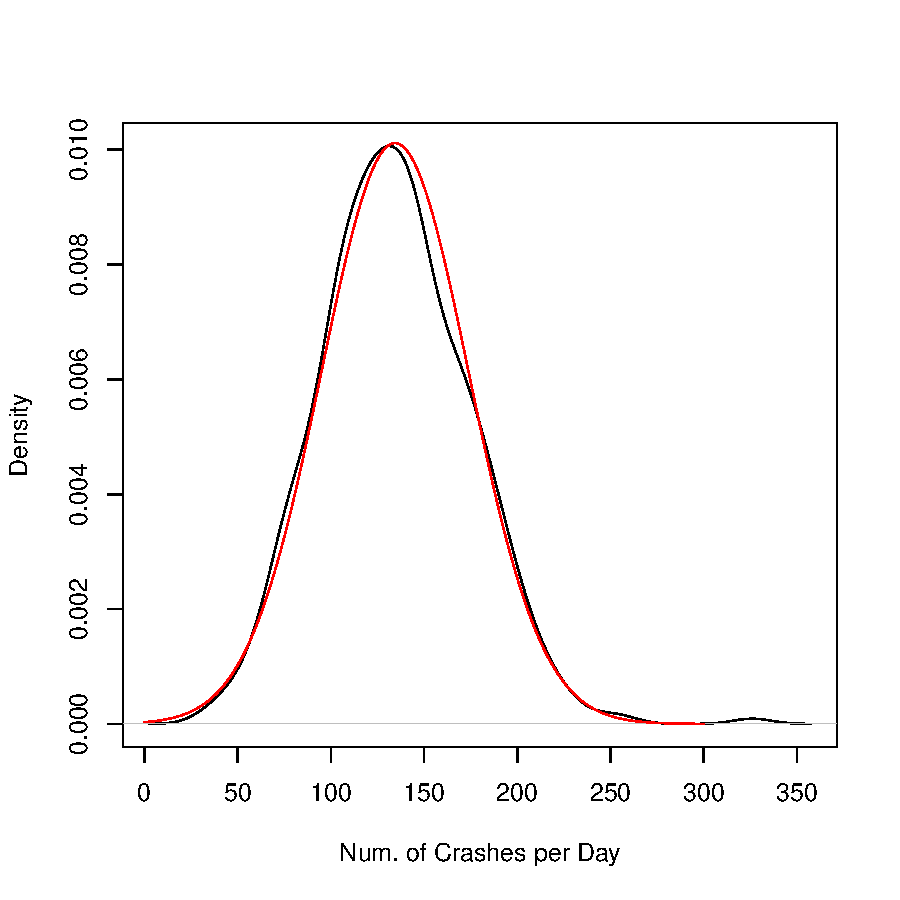
\includegraphics{regression-005}



\pagebreak
\subsection{Non-parametric Approach}




\pagebreak
\subsection{Random Forest}







\pagebreak
\section{Answering Hypotheses}


1. Visibility on a given day will be inversely correlated with \# of crashes per day.

2. Temperature will have a weak correlation with \# of crashes per day (people drive more recklessly in the summer? also tourism = more traffic in summer). 

3. Precipitation will be correlated with \# of crashes per day. 

4. Summer will have more crashes involving cyclists and motorcyclists. 

5. Crash fatality will be higher on weekends when more people are driving under the influence. 

6. Fatal, more severe crashes occur proportionately more often at nighttime, as visibility is reduced due to lack of sunlight. 

8. Single-vehicle crashes should be more proportionally higher during adverse weather, especially snow/ice conditions. 



\end{document}
